% PGFPlots: 3D surface and contour plots
\documentclass{article}
\usepackage{pgfplots}
\pgfplotsset{compat=1.18}
\usepgfplotslibrary{colormaps}

\begin{document}

% --- Surface plot ---
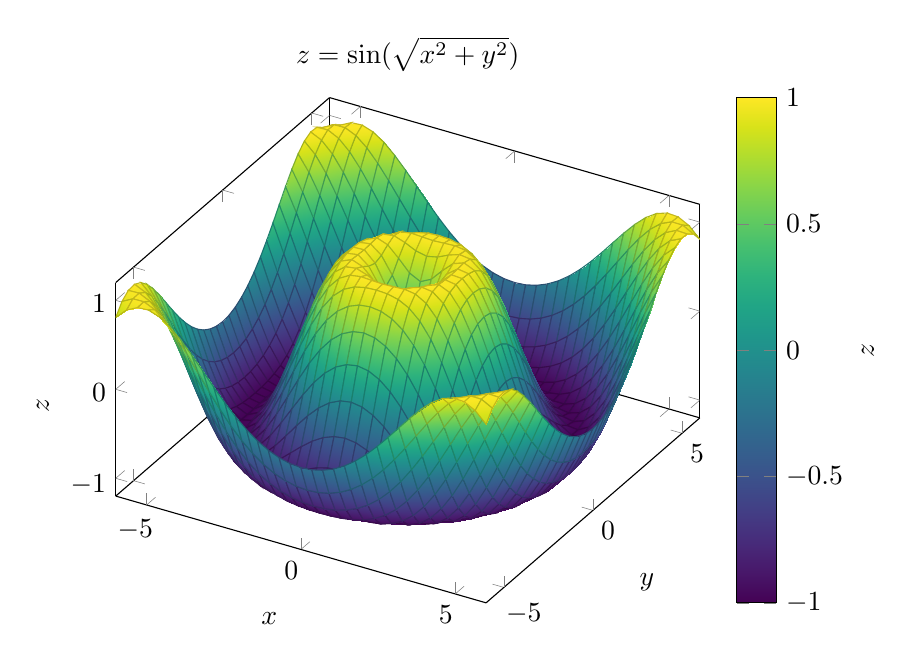
\begin{tikzpicture}
  \begin{axis}[
    view={30}{45},
    width=9cm, height=8cm,
    xlabel={$x$}, ylabel={$y$}, zlabel={$z$},
    colormap/viridis,
    colorbar,
    colorbar style={ylabel={$z$}},
    title={$z = \sin(\sqrt{x^2+y^2})$},
  ]
    \addplot3[
      surf,
      shader=faceted interp,   % smooth shading with visible grid
      domain=-6:6,
      y domain=-6:6,
      samples=35,
    ] {sin(deg(sqrt(x^2+y^2)))};
  \end{axis}
\end{tikzpicture}

\bigskip

% --- Contour (filled) plot ---
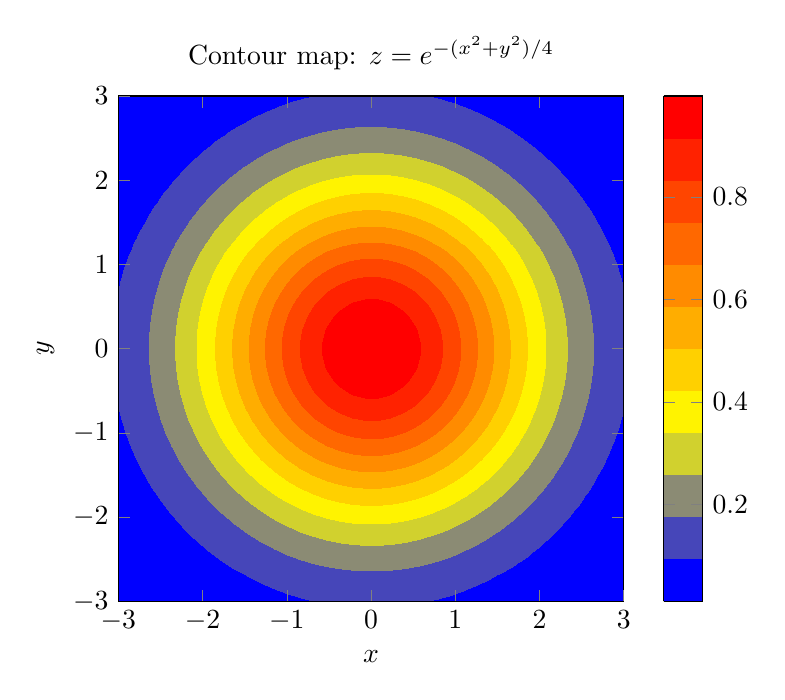
\begin{tikzpicture}
  \begin{axis}[
    view={0}{90},              % top-down = contour map view
    width=8cm, height=8cm,
    xlabel={$x$}, ylabel={$y$},
    colormap/hot,
    colorbar,
    title={Contour map: $z = e^{-(x^2+y^2)/4}$},
  ]
    \addplot3[
      contour filled={number=12},
      domain=-3:3,
      y domain=-3:3,
      samples=40,
    ] {exp(-(x^2+y^2)/4)};
  \end{axis}
\end{tikzpicture}

\end{document}
